\documentclass[../main.tex]{subfiles}
\graphicspath{{\subfix{../images/}}}

\begin{document}
% Explain how the requirements you have defined in the RASD map to the design elements that you have defined in this document
In this section, the mapping between the requirements specified in the RASD and the components of the eMall system is shown. To all the components abbreviations are given:
\begin{itemize}
    \item \textbf{CA} - ClientApp
    \item \textbf{AS} - AccessService
    \item \textbf{UM} - UserManager
    \item \textbf{DS} - DriverService
    \item \textbf{GM} - GeolocationManager
    \item \textbf{BM} - BookingManager
    \item \textbf{PM} - PaymentManager
    \item \textbf{SuM} - SuggestionManager
    \item \textbf{OS} - OperatorService
    \item \textbf{SM} - StationManager
    \item \textbf{CM} - ChargeManager
    \item \textbf{EM} - EnergyManager
    \item \textbf{NM} - NotificationManager
    \item \textbf{DM} - DataManager
    \item \textbf{DB} - DBMS
    \item \textbf{MAP} - MapService
    \item \textbf{CalS} - CalendarService
    \item \textbf{NavS} - NavigationService
    \item \textbf{VeS} - VehicleSensors
    \item \textbf{BankS} - BankService
    \item \textbf{SocS} - SocketSensor
    \item \textbf{BattS} - BatterySensor
    \item \textbf{DSO} - DSOPublisher
\end{itemize}
\begin{center}
\begin{longtable}{| c | p{9cm} | p{5cm} | } 
\hline
\textbf{Id} & \textbf{Description}  & \textbf{Components}\\
\hline
R1 & The system shall allow an unregistered Driver to register and create an account & CA, AS, UM, DM, DB\\ 
\hline
R2 & The system shall allow a registered Driver to log into his account & CA, AS, UM, DM, DB\\
\hline
R3 & The system shall allow a registered Driver to delete his account  & CA, AS, UM, DM, DB\\
\hline
R4 & The system shall allow a registered Driver to add one or more vehicles to his account 
 & CA, AS, UM, DM, DB\\
\hline
R5 & The system shall allow a registered Driver to delete one or more vehicles from his account
 & CA, AS, UM, DM, DB\\
\hline
R6 & The system shall allow a registered Driver to book a charging slot of a station for a certain time frame
& CA, AS, UM, DS, BM, SM, DM, DB\\
\hline
R7 & The system shall allow a registered Driver to acquire information of a selected charging station
& CA, AS, UM, DS, GM, DM, DB\\
%\hline
%R8 & The system shall allow a registered Driver to book a charge in a charging station in a certain time frame\\
\hline
R8 & The system shall allow a registered Driver to visualise the details of his charging process & CA, AS, UM, DS, BM, CM, DM, DB\\
\hline
R9 & The system shall allow a registered Driver to visualize the current offers of charging stations
& CA, AS, UM, DS, GM, DM, DB\\
\hline
R10 & The system shall allow a registered Driver to pay for the obtained service through an external API
& CA, AS, UM, DS, BM, CM, PM, DM, DB, BankS\\
\hline
R11 & The system shall allow a registered Driver to cancel a reservation 
& CA, AS, UM, DS, BM, DM, DB\\
\hline
R12 & The system shall not allow a registered Driver to book for a charge when he has already a reservation
& CA, AS, UM, DS, BM, DM, DB\\
\hline
R13 & The system shall allow a registered Driver to know about his actual position and nearby charging stations through an external API
& CA, AS, UM, DS, GM, DM, DB, MAP\\
\hline
R14 & The system shall allow an Operator working for the CPO to log into his account
& CA, AS, UM, DM, DB\\
\hline
R15 & The system shall allow a registered Operator to create an offer to the charging station managed by him
& CA, AS, UM, OS, SM, DM, DB\\
\hline
R16 & The system shall allow a registered Operator to modify the charging source of the charging station managed by him
& CA, AS, UM, OS, SM, EM, DM, DB, DSO, BattS\\
\hline
R17 & The system shall allow a registered Operator to modify the price of the energy of a charging station managed by him
& CA, AS, UM, OS, SM, DM, DB\\
\hline
R18 & The system shall allow a registered Operator to check the status of the charging station managed by him
& CA, AS, UM, OS, SM, EM, DM, DB, BattS\\
\hline
R19 & The system shall allow a registered Operator to visualise data provided by DSOs
& CA, AS, UM, OS, SM, EM, DM, DB, DSO\\
\hline
R20 & The system shall allow a registered Operator to choose from which DSO to acquire energy & CA, AS, UM, OS, SM, EM, DM, DB, DSO, BattS
\\
\hline
R21 & The system must be able to decide automatically where to get energy for charging & SM, EM, DM, DB, DSO, BattS
\\
\hline
R22 & The system must be able to notify the Driver when the charging process starts & CA, AS, UM, DS, BM, CM, DM, DB, SocS
\\
\hline
R23 & The system must be able to notify the Driver when the charging process ends & CA, AS, UM, CM, NM
\\
\hline
R24 & The system must be able to suggest the Driver to charge the vehicle, the suggestion is based on information retrieved through external APIs & CA, AS, UM, DS, SuM, NM, DM, DB, CalS, NavS, VeS\\
\hline
R25 & The system must be able to notify user in case of exceptions & CA, AS, UM, DS, GM, BM, PM,  OS, SM, CM, EM, DM, DB
\\
\hline
R26 & The system must be able to notify user on successful actions & CA, AS, UM, DS, GM, BM, PM,  OS, SM, CM, EM, DM, DB
\\
\hline
R27 & The system must be able to retrieve a map through an external API & CA, AS, UM, MAP
\\
\hline
R28 & The system shall allow a registered Driver to start his charge & CA, AS, UM, DS, BM, CM, DM, DB, SocS
\\
\hline
R29 & The system shall allow a registered Driver to finish his charge & CA, AS, UM, DS, BM, CM, PM, DM, DB, BankS
\\
\hline
\end{longtable}
\end{center}

\begin{figure}[H]
    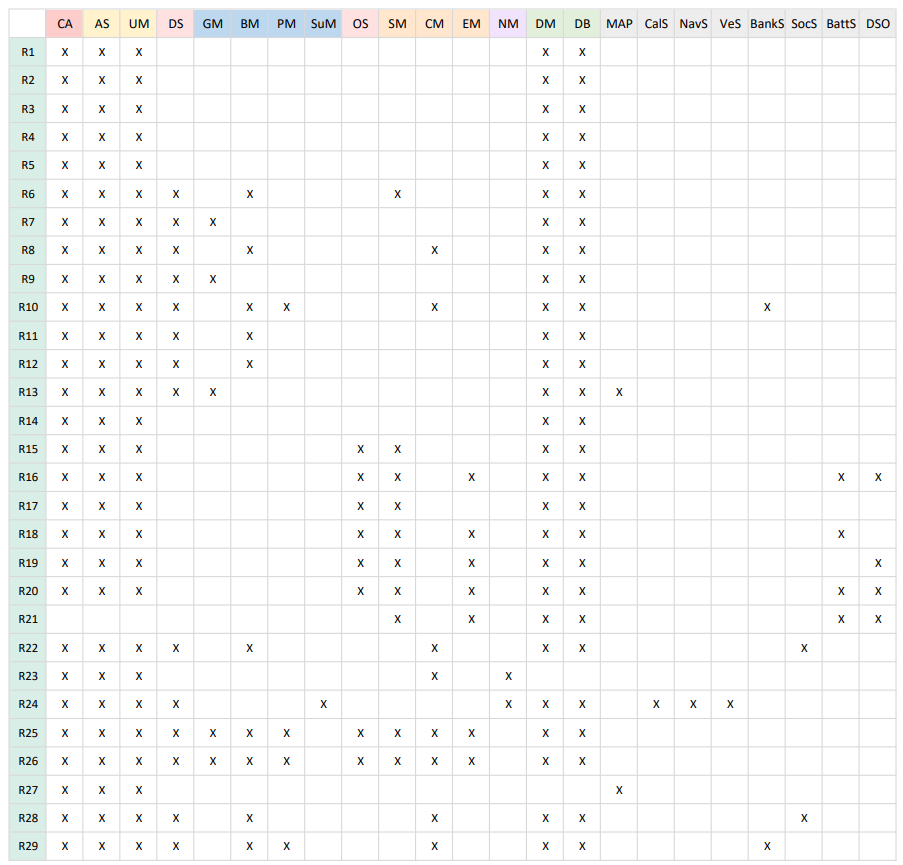
\includegraphics[width=1.05\textwidth]{images/Traceability.png}
    \caption{Table of Requirements Traceability}
    \label{fig:traceability}
\end{figure}

\end{document}